% -*- coding: utf-8 -*-

\documentclass[b5paper,papersize,tombow,12pt]{jsbook}

\usepackage{amsmath,ascmac}
\usepackage{graphicx}
\usepackage{lettrine}
\usepackage{fancyhdr}
% Palatino
\usepackage{palatino}


%% Page Layout
% B5: 182mm x 257mm
\setlength{\voffset}{0mm}
\setlength{\topmargin}{-15mm}
\setlength{\textheight}{29\Cvs}
\setlength{\footskip}{10mm}

% set margin for openleft
% \setlength{\oddsidemargin}{-\oddsidemargin}
% \setlength{\evensidemargin}{-\oddsidemargin}


\pagestyle{fancy}

\fancyhead{}
% \fancyhead[RO,RE]{\rightmark}
% \fancyhead[LE,LO]{\leftmark}
\fancyhead[RO]{\rightmark}
\fancyhead[LE]{\leftmark}
\cfoot{\bfseries -- \thepage \ --} % page number at the center bottom
\renewcommand{\headrule}{
\vskip -1.5mm
\hskip-0.03\textwidth\includegraphics[width=1.06\textwidth,height=3.78mm]{hayamiz/images/hrule.eps}
\vskip -2.28mm
}

% jsbook.cls use 'plainhead' style for the first page of each chapter
\fancypagestyle{plainhead}{
\fancyhf{}
\cfoot{\bfseries -- \thepage \ --}
\renewcommand{\headrulewidth}{0.0pt}
\renewcommand{\headrule}{}
}

% jsbook.cls use 'empty' style for blank
\fancypagestyle{empty}{
\fancyhf{}
\cfoot{\bfseries -- \thepage \ --}
\renewcommand{\headrulewidth}{0.0pt}
\renewcommand{\headrule}{}
}

\makeatletter
\renewcommand{\chapter}{%
  \if@openright\cleardoublepage\else\clearpage\fi
  \plainifnotempty % 元: \thispagestyle{plain}
  \global\@topnum\z@
  \if@english \@afterindentfalse \else \@afterindenttrue \fi
  \secdef\@chapter\@schapter}
\def\@chapter[#1]#2{%
  \ifnum \c@secnumdepth >\m@ne
    \if@mainmatter
      \refstepcounter{chapter}%
      \typeout{\@chapapp\thechapter\@chappos}%
      \addcontentsline{toc}{chapter}%
        {\protect\numberline
        {\if@english\thechapter\else\@chapapp\thechapter\@chappos\fi}%
        #1}%
    \else\addcontentsline{toc}{chapter}{#1}\fi
  \else
    \addcontentsline{toc}{chapter}{#1}%
  \fi
  \chaptermark{#1}%
  \addtocontents{lof}{\protect\addvspace{10\p@}}%
  \addtocontents{lot}{\protect\addvspace{10\p@}}%
  \if@twocolumn
    \@topnewpage[\@makechapterhead{#2}]%
  \else
    \@makechapterhead{#2}%
    \@afterheading
  \fi}
\def\@schapter#1{%
  \chaptermark{#1}%
  \if@twocolumn
    \@topnewpage[\@makeschapterhead{#1}]%
  \else
    \@makeschapterhead{#1}\@afterheading
  \fi}

\def\@normalchapter[#1]#2{%
  \ifnum \c@secnumdepth >\m@ne
    \if@mainmatter
      \refstepcounter{chapter}%
      \typeout{\@chapapp\thechapter\@chappos}%
      \addcontentsline{toc}{chapter}%
        {\protect\numberline
        {\if@english\thechapter\else\@chapapp\thechapter\@chappos\fi}%
        #1}%
    \else\addcontentsline{toc}{chapter}{#1}\fi
  \else
    \addcontentsline{toc}{chapter}{#1}%
  \fi
  \chaptermark{#1}%
  \addtocontents{lof}{\protect\addvspace{10\p@}}%
  \addtocontents{lot}{\protect\addvspace{10\p@}}%
  \if@twocolumn
    \@topnewpage[\@makechapterhead{#2}]%
  \else
    \@makechapterhead{#2}%
    \@afterheading
  \fi}
\def\@normalschapter#1{%
  \chaptermark{#1}%
  \if@twocolumn
    \@topnewpage[\@makeschapterhead{#1}]%
  \else
    \@makeschapterhead{#1}\@afterheading
  \fi}
\def\@makechapterhead#1{%
  {\parindent \z@ \raggedright \normalfont
    \ifnum \c@secnumdepth >\m@ne
      \if@mainmatter
        \huge\headfont \@chapapp\thechapter\@chappos
        \par\nobreak
        \vskip \Cvs % 欧文は20pt
      \fi
    \fi
    \interlinepenalty\@M
    \begin{center}
     {\LARGE \headfont #1}\par\nobreak\noindent
\hskip-0.03\textwidth\includegraphics[width=1.06\textwidth,height=7.59mm]{hayamiz/images/chapter-title-ornament.eps}\vskip-7.59mm\vskip-0.5\Cvs
    \end{center}
    \par\nobreak
    \vskip 1\Cvs}} % 欧文は40pt
\def\@makeschapterhead#1{%
  {\parindent \z@ \raggedright
    \normalfont
    \interlinepenalty\@M
	\begin{center}
    {\LARGE \headfont #1}\par\nobreak\noindent
\hskip-0.03\textwidth\includegraphics[width=1.06\textwidth,height=7.59mm]{hayamiz/images/chapter-title-ornament.eps}\vskip-7.59mm\vskip-0.5\Cvs
    \end{center}
	\par\nobreak
    \vskip 3\Cvs}} % 欧文は40pt
\makeatother

\renewcommand{\prechaptername}{Article }
\renewcommand{\postchaptername}{}

\ifx\Cht\undefined
 \newdimen\Cht\newdimen\Cdp
 \setbox0\hbox{\char\jis"2121}\Cht=\ht0\Cdp=\dp0\fi
\makeatletter
\long\def\linespace#1#2{\par\noindent
  \dimen@=\baselineskip\multiply\dimen@ #1\advance\dimen@-\baselineskip
  \advance\dimen@-\Cht\advance\dimen@\Cdp
  \setbox0\vbox{\noindent #2}\advance\dimen@\ht0\advance\dimen@-\dp0%
  \vtop to\z@{\hbox{\vrule width\z@ height\Cht depth\z@
   \raise-.5\dimen@\hbox{\box0}}\vss}%
  \dimen@=\baselineskip\multiply\dimen@ #1\advance\dimen@-\baselineskip
  \vskip\dimen@}
\makeatother

\title{Database Times Vol. 1}
\date{2012/8/11}
\author{Hotchpotch Society}

\begin{document}

\thispagestyle{empty}

\frontmatter

% タイトルページ
\begin{center}
 \includegraphics[width=12cm]{hayamiz/images/title.eps}
 \par\vspace*{50mm}
 \noindent Hotchpotch Society
\end{center}

% まえがきページ
% -*- coding: utf-8 -*-

\chapter*{まえがき}
\addcontentsline{toc}{chapter}{まえがき}
\thispagestyle{plainhead}

The Database Times vol.1 をお手にとっていただきありがとうございます。

本書は、データベースシステムを中心として、様々な情報技術に関する話題を読
者の皆様にお届けすることを目的としています。みなさんは「データベースシス
テム」というものにどのようなイメージをお持ちでしょうか。SQLを投げるとデー
タを返してくれる、なんだかよくわからないけれど枯れた時代遅れの技術だとい
うイメージを持っている人が多いのではないかと思います。

しかしながら、実際のデータベースシステムは古の技術を土台として、その時代
の最先端の技術が詰め込まれた非常に魅力的な技術の集大成なのです。世界中で
生み出されるデータ量がどのくらいかご存知でしょうか。2010年までに生み出さ
れたデータ量はなんと1,227ペタバイト。しかも、2020年には7,910,000ペタバイ
トになるであろうと予測されています。人類が産み出そうとしているデータ量は、
まさに爆発的な勢いで増え続けています。このデータの膨張を支える縁の下の力
持ちがデータベースシステムです。加速するデータ量の増加に伴って、データベー
スも日々進歩を続けているのです。

そんなデータベースシステムが、どのようにして生まれ、そして最近ではどんな
ことが話題になっているのか、データベースシステムの今と昔に迫るのが本書の
目指すところです。

\begin{flushright}
 2012年 8月

Hotchpotch Society
\end{flushright}

\newpage

\subsection*{お品書き}

\noindent {\bf ■ データベースシステムの夜明け}

今の世の中、データベースシステムといえばリレーショナルデータベースシステ
ムです。そのリレーショナルデータベースシステムが、一体どのようにして生み
出されたのか、そしてどのように発展を遂げていったのか、その歴史を辿ります。

\vspace*{\Cvs}

\noindent {\bf ■ PostgreSQLカンファレンス2012 レポート}

オープンソースDBMS代表格の一つであるPostgreSQLは、最近は業務でも用いられ
ることがかなり増えてきているようです。そんな PostgreSQL の最新技術事情に
触れられる PostgreSQL カンファレンスの参加レポートをお届けします。

\vspace*{\Cvs}

\noindent {\bf ■ とある世界で一番高速なBrainfuckインタプリタ}

近年ではSAP HANAやMemSQLなどの主記憶データベースが話題となっているように、
膨大するデータ量を捌ききるための「速さ」が強く求められています。データベー
スシステムはSQLというプログラミング言語の処理系という側面も持ちあわせてお
り、言語処理系の高速な実装はデータベースシステムには必要不可欠です。言語
処理系をいかに高速にするのか、その技術について世界最速Brainfuckインタプリ
タの実装者が解説します。

\vspace*{\Cvs}

\noindent {\bf ■ クラウド時代のDNS}

\noindent {\bf ■ IPv4がこの先生きのこるには}

最近では「クラウド」という言葉が話題となっていますが、その背景にはもはや
単一のコンピュータだけでシステムを構築してすべてがうまくいく時代は終焉を
迎え、ネットワークによりコンピュータを有機的に結合することが必須となりつ
つある現代の技術トレンドがよみとれます。ネットワーク技術では今一体何が起
きているのか、その最前線に迫ります。

\vspace*{\Cvs}

\noindent {\bf ■ 電算機技能者的同人誌執筆環境構築概論}

本書は \LaTeX で執筆されています。プログラマが \LaTeX で本を書くというの
はどういうことなのか、その開発(執筆)環境を紹介します。


\thispagestyle{plainhead}


% 目次ページ
\setcounter{tocdepth}{0} % show only chapters
\tableofcontents

\mainmatter

\pagestyle{fancy}

% 本文ここから
% -*- coding: utf-8 -*-

\chapter{PostgreSQLカンファレンス2012 レポート}

\begin{flushright}
 {\headfont はやみず}
\end{flushright}

2012年3月24日に日本PostgreSQLユーザ会主催で開催されたPostgreSQLカンファレ
ンス2012に参加してきました。この記事は,PostgreSQLカンファレンス全体の概
観についてレポートを記したものです。

このカンファレンスは技術的な話題を中心として,PostgreSQLに関する導入事例
や技術的な話題を提供するためのカンファレンスです。 昨年度の参加者約180名
に対して今年度は275名(関係者含む)ということで,日本におけるPostgreSQLのユー
ザ層の広がりを感じさせます。 特にこの数年はビジネスとしてこのカンファレン
スに参加する方も増えているそうで,業務用途としてのPostgreSQLの利用が広まっ
ていることを示しているのではないかと思われます。

Linuxの急速な普及をきっかけとして,今やオープンソースソフトウェアを業務に
おいて利用することは全く珍しくなくなっています。 PostgreSQLもその例に漏れ
ず,といったところでしょうか。本年度のカンファレンスのプログラムも,業務
用途におけるPostgreSQLの利用ということが一つの大きな軸として捉えられてい
るように見えます。 例えば,午後のプログラムは3トラック構成となっていたの
ですが,そのうちの1トラックは「マイグレーショントラック」と題して他の
DBMSからPostgreSQLへ移行することを主眼としたものであり,「商用 DB から
PostgreSQL への移行」「PostgreSQL がより使いやすく進化した Postgres Plus
Advanced Server の実力とは」などは明らかに商用DBを意識しています。また,
技術トラックやLightning Talkにおいて高可用・高性能なPostgreSQLクラスタに
関する発表がありました。業務用DBMSとしてはクラスタソリューションがほしい。
MySQLにはMySQL Clusterが,OracleにはOracle RACが,じゃあPostgreSQLはどう
なの?というポイントに答えを出すのが,今回のカンファレンスの一つの見所だっ
たのではないでしょうか。

もちろん,ビジネス的な側面だけではなく,技術の深い話もできるのがこのカン
ファレンスの魅力だと思います。午前中の基調講演では,PostgreSQLの大型移行
案件の事例紹介であるフランス社会保障機構の講演に加えて,PostgreSQLのコア
開発者でありコミュニティの中でも若手のエースと目されているEnterpriseDB社
のRobert Haas氏によるPostgreSQL 9.2の新機能に関する講演がありました。こち
らの講演では,メニーコア環境におけるスケーラビリティ向上の取り組みや,
Index-only Scanの導入,消費電力削減のための実装努力,レプリケーションの新
機能,その他細々とした新機能などが紹介されました。加えて,バージョン9.2よ
り後にどんな技術的な課題に取り組んでいくべきか,といった方向性についても
触れられていました。質疑応答も非常に活発に行われていたのが印象的です。一
つ残念だったのは,こちらの講演は発表・質疑応答ともに逐次翻訳が行われてい
たため,実際に話せる時間が半分になってしまっていたことです。英語のみで進
行してくれたほうが個人的には中身がもっと詰まって面白かったのではないかと
思いますが,難しいところですね。

もう1件技術的な講演として面白かったのは藤井雅雄氏,松尾隆利氏による
「PostgreSQL 9.1 同期レプリケーションと Pacemaker による高可用クラスタ化
の紹介」です。 こちらの発表では,まず藤井氏からPostgreSQLにおけるレプリケー
ションの詳細について紹介されていました。非同期レプリケーション,同期レプ
リケーションの動作や,何ができるのか,何ができないのかについて丁寧にまと
められており,レプリケーション機能の全体像を理解できる発表でした。またそ
れに加えて,9.2で導入される予定のレプリケーション関連の機能紹介や,周辺ツー
ルに関する紹介もありました。 その後,松尾氏により同期レプリケーション機能
とPacemakerを組み合わせることによる,障害発生時にもフェイルオーバ可能なク
ラスタ構成法についての発表が行われました。Pacemakerについては名前くらいし
か知らなかったのですが,障害発生からフェールオーバまでの流れがわかりやす
く図解されており,Pacemakerを知るという観点からも有用な発表であったように
思います。

本会議のほうについてはこんなところで,懇親会にも参加したのでの話をひとつ。
PostgreSQLのお役立ち情報源として参照している人も多いかと思われるLet's
Postgresという読み物サイトがあるのですが,こちらの運営をしている方とお話
をさせて頂きました。 この手の読み物サイトでは,最も需要の高い入門系記事や,
企業の提灯記事が並ぶというのがよくあるパターンなのですが,Let's Postgres
にはPostgreSQLの内部構造についてやたら詳しく書かれた記事がたくさんあり,
これは一体どういったことだろうと思っていたのでした。 そのことを聞いてみた
ところ,内部構造の多くは記事PostgreSQL本体にコミットしている開発者の方々
が好きで寄稿しているということだそうです。PostgreSQL自体が内部構造まで含
めた子細なドキュメントが充実していますが,新機能の実装詳解がこれほどまで
精力的に行われているソフトウェアはなかなかないのではないかとおもいます。
これらの記事は目的別ガイド:内部解析編としてまとめられています。内部の詳
解に加えて,開発プロセスへの参加方法についても紹介されており,非常に充実
した内容となっています。PostgreSQLの中身に興味がある人は必見ですね。

以上,簡単ではありますが参加レポートでした。

% TODO: もっと書く

% -*- coding: utf-8 -*-

\cleardoublepage
\plainifnotempty

\chapter{データベースシステムの夜明け}

\begin{flushright}
はやみず
\end{flushright}

\lettrine{デ}ータベースシステム無しでは、今日の社会は成り立たないと言って
良いでしょう。社会が高度に情報化された現在、世界中で大量のデジタルデータ
が日々生み出され、飛び交い、消費され、そして蓄積されてゆきます。2011年に
人類の生み出したデータ量は1,800ペタバイトにのぼります。一方で、膨大なデジ
タルデータは、単に生み出され、蓄積されてゆくだけではただのゴミも同様です。
必要なときに必要なデータが取り出せるよう、適切に管理してゆかなければなり
ません。そのための根幹たる存在が、データベースシステムなのです。

みなさんが馴染みのあるであろう MySQL や PostgreSQL、あるいは Oracle といっ
たデータベースシステムは、正確には「リレーショナルデータベースシステム」
と呼ばれています。リレーショナルデータベースシステムの歴史を辿ると、その
起源はある一篇の論文に遡ることができます。

その論文こそが、Edgar F.  Coddにより1970年に発表された ``A Relational
Model of Data for Large Shared Data Banks'' です。この論文は、リレーショ
ナルデータベースの最も重要な基礎となる{\bf リレーショナルデータモデル}を
提唱したもので、いわばデータベースシステム分野における金字塔です。古典力
学を Newton が拓き、相対性理論を Einstein が拓いたとするならば、データベー
スにおける一大分野であるリレーショナルデータベースを拓いたのは間違いなく
Edgar Codd その人といって間違いないでしょう。

そして、Codd によりリレーショナルモデル提唱から数年の後に、UNIXで動作する
世界初のリレーショナルデータベースシステムの開発プロジェクトが立ち上がり
ます。Michael Stonebraker率いる{\bf INGRESプロジェクト}です。Coddにより確
立されたリレーショナルデータベースシステムの基礎理論を、実際に動くソフト
ウェアとして実現し、そしてそれを世に広めたのがINGRESなのです。

本稿では、Coddによるリレーショナルデータモデルの提唱から、INGRESプロジェ
クトの黎明期の記録を辿り、現代の社会を支えるデータベースシステムがいかに
して創り上げられたのか、その歴史を紐解いてみようと思います。

{\small ※ これ以降、特に断りのない場合、リレーショナルデータベースシステムを指して
単にデータベースシステムと書くことがあります。}

\section{時代はリレーショナルへ}

1960年代以前のデータベースシステムは階層型データモデル、やネットワーク型
データモデルというデータモデルに基づいて構築されていました。

\begin{figure}[tb]
 \begin{minipage}{0.48\textwidth}
  \begin{center}
   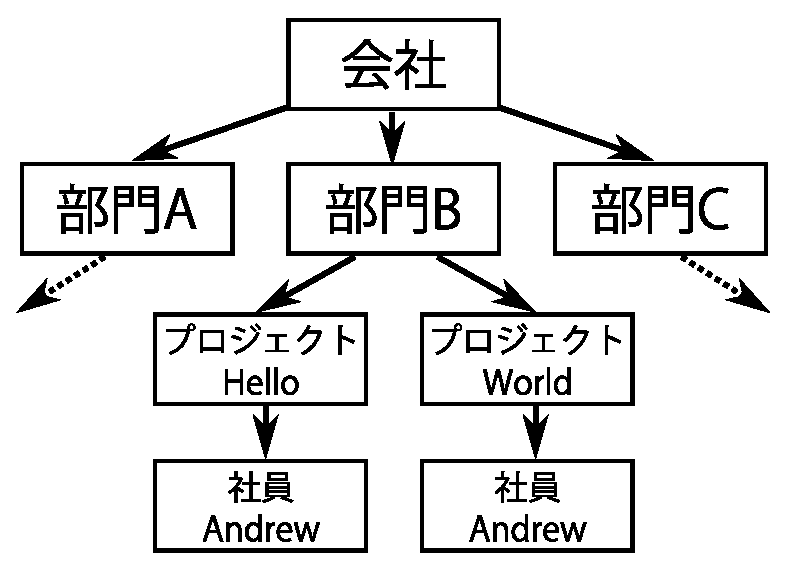
\includegraphics[width=5cm]{hayamiz/images/hierarchical-data-model.eps}
   \caption{階層型データモデル}
   \label{214539_12Jul12}
  \end{center}
 \end{minipage}
 \begin{minipage}{0.48\textwidth}
  \begin{center}
   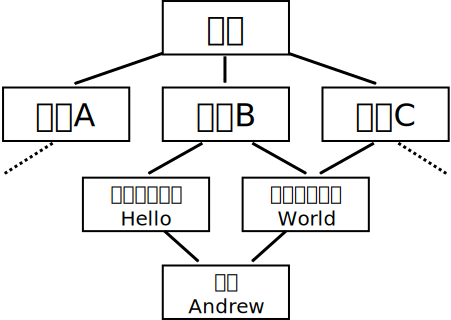
\includegraphics[width=5cm]{hayamiz/images/network-data-model.eps}
   \caption{ネットワーク型データモデル}
   \label{214707_12Jul12}
  \end{center}
 \end{minipage}
\end{figure}

階層型データモデルというのは、木構造を用いてデータを組織化したデータモデ
ルです。たとえば会社組織を階層型データモデルで表そうと思うと、会社の下に
は複数の部門が属しており、各部門の下には複数のプロジェクトがあり、各プロ
ジェクトの下には社員が属している、というようにスキーマを定義してゆきます
(図\ref{214539_12Jul12})。ここで、例えば2つのプロジェクトHelloとWorldに属
する1人の社員Andrewがいたとしたらどうでしょう。階層型データモデルでは、あ
るデータの実体(ここでは1人の社員)は親となるデータの実体(プロジェクト)
を複数持つことができません。そのため、各プロジェクトごとにAndrewのデータ
を持つことになり、データの重複が生じてしまいます。また、部門Bと部門Cが共
同でプロジェクトWorldを運営していることを表現しようと思うと、プロジェクト
のデータに加えてその下にぶら下がっている社員のデータも併せてコピーしなけ
ればなりません。このような欠点を克服したのがネットワーク型データモデルで
す(図\ref{214707_12Jul12})。ネットワーク型データモデルでは、データの実
体が複数の親を持つことができる有向グラフをデータ構造として採用したため、
前述のようなデータ重複の問題は発生しません。

ネットワーク型モデルによりより一般的なデータ構造を表現できるようにはなり
ました。しかし、階層型モデルやネットワーク型モデルに基づくデータベースは、
データのアクセスに一つ大きな問題を抱えていました。これらのデータベースに
おいてデータの問い合わせを行う際には、データの構造がどのようになっている
かを把握し、そしてどのような手順でデータを取得するかを利用者が知っている
必要があったのです。例えば図\ref{214707_12Jul12}のデータベースにおいて社
員Andrewのデータを取得するためには、「会社のデータを読みとり、部門Bのデー
タを読み取り、プロジェクトHelloのデータを読み取り、社員Andrewのデータを読
み取る」という手順を指定してあげなければなりません。このように、欲しいデー
タにアクセスするための``how'' をもって問い合わせを行うデータベースシステ
ムは、ユーザがデータの案内(navigation)をするという意味で{\bf ナビゲーショ
ナルデータベースシステム}と呼ばれます。

もしもナビゲーショナルデータベースシステムにおいて、図
\ref{214707_12Jul12}の会社で組織改変があり、各部門の下には課が設置され、
その下にプロジェクトが属するという構造にデータベースが修正されたとしたら
どうなるでしょう。これまで社員のデータにアクセスするアプリケーションは会
社→部門→プロジェクト→社員とたどっていましたが、会社→部門→課→プロジェ
クト→社員とたどるように修正しなければなりません。このように、ナビゲーショ
ナルデータベースシステムでは、ある特定のデータのみに興味があったとしても、
その上位構造に変化があった時にはデータにアクセスする方法を再構成しなけれ
ばなりませんでした。

歴史的には、階層型モデルはそのシンプルさ故に初期のデータベースシステムに
おいて採用され、その後により一般的なデータの組織化を行うことができるよう、
ネットワーク型モデルが発明されます。1969年にはCODASYLという委員会によって、
ネットワーク型データモデルの標準化が行われ、データベースシステムの情勢は
階層型モデルからネットワーク型モデルに移るかと思われました。

そこに登場したのが、1970年\footnote{正確にはリレーショナルデータモデルの
論文は1969年にIBMの社内技術報に掲載され、翌1970年に米国コンピュータ学会の
論文誌に掲載されます。}にCoddによって提唱されたリレーショナルデータモデル
です。リレーショナルデータモデルは、数学の集合論に基づいてデータを組織化
する方法論であり、階層型モデルやネットワーク型モデルのようにデータアクセ
スのための具体的なアルゴリズムを内包しません。ユーザは「どんなデータが欲
しいか」を記述するたけで、具体的なアクセス方法はデータベース側が判断して
データを取得することができます。つまり、ナビゲーショナルデータベースシス
テムでは ``how'' を与えなければデータのアクセスが行えなかったのですが、リ
レーショナルデータベースは ``what'' を与えるだけでデータのアクセスが可能
となります\footnote{リレーショナルモデルの数学的な定義や、なぜそれにより
``what''でデータの問い合わせが可能となるのかの説明については、それだけで
一冊の本になってしまうので他書に譲ります。}。

また階層型モデルなどとは異なり、リレーショナルモデルはしっかりとした数学
的基礎の上に成り立っており、後のデータベースシステム研究の大きな基盤とな
りました。これまでプログラマによるある種の職人芸の上に成り立っていたデー
タベースシステムは、リレーショナルデータモデルの登場によって科学の領域へ
と押し上げられたのです。

ちなみに、データベースのお勉強をした人たちは、ドメイン、リレーション、タ
プル、主キー、外部キー、○○正規形という言葉に聞き覚えがあるかもしれませ
んが、これら教科書に載っているリレーショナルデータモデルのかなりの部分が
1970年の論文の段階で体系的にまとめられています。もちろん現在のリレーショ
ナルデータモデルは様々な改良が加えられていますが、その基本的な骨子はほぼ
そのままの形で残っています。この論文はタイトルで検索すればオンラインで読
むことができます。自分の勉強した知識と照らし合わせながら読んでみると面白
いのではないでしょうか。

\section{データベースシステムの産声}

UC Berlekey で INGRESプロジェクト始まる

System R ?

\section{つぎに}


\section*{参考文献}

\begin{itemize}
 \item E. F. Codd, ``A Relational Model of Data for Large Shared Data
       Banks'', {\it Communications of the ACM}, Vol. 13, No. 6, (1970.06)
\end{itemize}
% -*- coding: utf-8 -*-

\chapter{嘘を嘘と見抜きたい人のためのマイクロベンチマーク入門}

\begin{flushright}
 はやみず
\end{flushright}

\section{プロローグ}

先日、ちょっとしたハプニングがありました。

研究室で共用マシンとしてMacbook pro 17インチ買いましょうということになり、
僕が細かい仕様決定から発注までを担当しました。幸い予算はそれなりに余裕が
あったので、メモリもCPUも一番上のオプションを選び、標準のハードディスク
750GBのかわりにSSD 500GBを選択するなど、贅を尽くしたMacbook proを注文して、
届くのをいまかいまかと待っていました。ちなみに、HDDをSSDにするだけでお値
段が9万円くらい跳ね上がります。

発注から2週間ほど待たされて、ようやくMacbook proが到着しました。

% -*- coding: utf-8 -*-

\chapter*{ドワンゴエンジニアの平凡な日常}

\lettrine{ま}
た私は如何にしてニコニコ静画(電子書籍)
のFlash版プレイヤーを200\%高速化したか

もしくは世界最速のBrainf*ckインタプリタがどうしたこうしたとか。

または国からお金を貰って毒にも薬にもならないものを作った
黒歴史について。

% 本文ここまで

\backmatter

\chapter{あとがき}
\pagestyle{empty}

あとがき
あとがき
あとがき
あとがき
あとがき
あとがき
あとがき
あとがき
あとがき
あとがき
あとがき
あとがき
あとがき
あとがき
あとがき
あとがき
あとがき
あとがき
あとがき

\newpage

\section*{著者紹介}

\noindent {\gt ■ はやみず}

駒場にある某研究室にて、データベースシステムと戯れる日々を過ごしている大
学院生。飽きっぽい性格。学部生のころはLisp系言語に傾倒したり、マルチコア
向け並列処理フレームワークの研究をしたりしていた。

\noindent {\gt ■ はやみず}

日本人。

\noindent {\gt ■ はやみず}

日本人。

\noindent {\gt ■ mmk (表紙デザイン)}

日本人。


\vspace*{50mm}

% 奥付
\begin{center}
 \includegraphics[width=8cm]{hayamiz/images/colophon.eps}
 \par\vspace*{1mm}
 \begin{tabular}{rl}
  \hline
  タイトル & Database Times vol.1 \\
  発行日 & 2012年8月11日 \\
  サークル & ホッチポッチソサイエティ \\
  著者 & はやみず、はやみず、はやみず、TODO: \\
  発行責任者 & はやみず \\
  連絡先 & {\it yuto+c82@hayamiz.com} or {\it @hayamiz} (Twitter) \\
  ウェブサイト & {\it http://hayamiz.com/\~{}hotchpotch/} \\
  印刷所 & TODO: \\
  \hline
 \end{tabular}
\end{center}

\end{document}
